\documentclass[11pt]{article}
\usepackage[T1]{fontenc}
\usepackage[utf8]{inputenc}
\usepackage{graphicx}
\usepackage{enumitem}
\usepackage{fancyhdr}
\usepackage{polski}

\pagestyle{fancy}
\fancyhead[L]{Kacper Achramowicz\\
Projekt indywidualny AiSD}
\fancyhead[R]{15.XI.2020\\
V1.0}
\begin{document}

\begin{huge}
\begin{center}
\textbf{Specyfikacja implementacyjna}
\end{center}
\end{huge}

 \renewcommand{\labelenumii}{\Roman{enumii}}
 \begin{enumerate}
 
 \item Informacje ogólne
 
 \begin{enumerate}[label=\arabic{enumi}.\arabic*.]
 
\item Forma przekazu\\
 Program wykonany jest w formie aplikacji działającej w terminalu. Do włączenia go wymagane jest posiadanie kompilatora Java. Program nie posiada dedykowanego GUI.
\item Sposób uruchomienia\\
 Aby włączyć program należy przejść w terminalu do katalogu zawierającego pilk wykonywalny \textbf{VaccOpt.jar} i włączyć go wpisując komendę \textsl{java -jar VaccOpt.jar "nazwaPliku"}, gdzie nazwaPliku to nazwa pliku z danymi. W przypadku wywołania bez argumentów program domyślnie korzysta z pliku \textsl{dane.txt}.
 \end{enumerate}
 
 
 
\item Opis pakietów\\
Pakiety zostały podzielone ze względu na funckjonalność.

\begin{enumerate}[label=\arabic{enumi}.\arabic*.]
 \item  Pakiet load\\
Głównym zadaniem tego pakietu jest wczytywanie danych z pliku. Klasa zawarta w tym pakiecie sprawdza, czy została podana nazwa pliku z danymi (jeżeli nie to otwiera plik "dane.txt").  Następnie sprawdza, czy format danych w pliku się zgadza.Dane w pliku muszą być oddzielone od siebie separatorem "|", a nazwy aptek i dystrybutorów nie mogą zawierać tego znaku. Każda z aptek musi mieć połączenie z każdym z dystrybutorów. Podaż musi być większa lub równa popytowi. Wszystke liczby zawarte w pliku muszą być liczbami dodatnimi, a zapotrzebowanie na szczepionki jak i ich dostępna ilość muszą być liczbami całkowitymi. Identyfikatory aptek muszą być unikatowe, tak samo musi być z identyfikatorami dystrybutorów, jednak zarówno apteka jak i dystrybutor mogą mieć to samo id (np. 0), ponieważ są innego typu. Możliwe informacje zwrotne o błędach:\\
- dane są źle sformatowane, separator "|" nie oddziela kolumn, lub występuje w nazwie apteki bądź dystrybutora \\
- co najmniej jedna z aptek nie jest połączona ze wszystkimi dystrybutorami,\\
- w pliku występują liczby ujemne,\\
- nie można potrzebować fragmentu szczepionki,\\
- podaż mniejsza od popytu,\\
- dublujące się ID apteki lub dystrybutora.\\
Na koniec dane są zapisywane do dwóch macierzy (tablic dwuwymiarowych). Jedna zawiera informacje o połączeniach aptek z dystrybutorami, druga o zapotrzebowaniu aptek i podaży dystrybutorów. \\
Przykładowy wygląd pliku danego jako input:\\
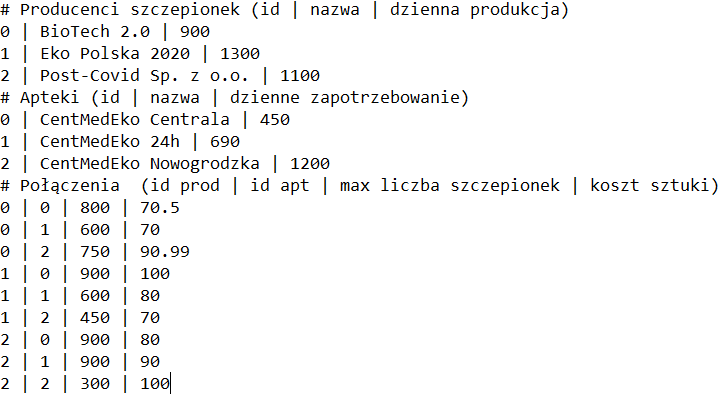
\includegraphics {in.png}
\item Pakiet aprox\\
Ten pakiet zawiera klasy, w których rozwiązywany jest trzon zadania oraz klasę main zawierającą tylko metodę main(). Ten pakiet spełnia dwa zadania:\\
- rozwiązuje główny problem przedstawiony w zadaniu metodą VAM (metoda aproksymacji Vogla),\\
- zawiera klasę, w której znajduje się metoda main(), w której wywoływane są najważniejsze metody pozostałych pakietów.\\
Tak naprawdę ten pakiet jest spoiwem łączącym cały program w jedną, działającą całość.
\item Pakiet save\\
W tym pakiecie znajduje się klasa, której zadaniem jest stworzenie i sformatowanie pliku $result.txt$. W tym pliku znajdują się informacje, które są wynikiem działań w pakiecie approx. Przykładowa struktura pliku $result.txt$ jest przedstawiona poniżej.\\
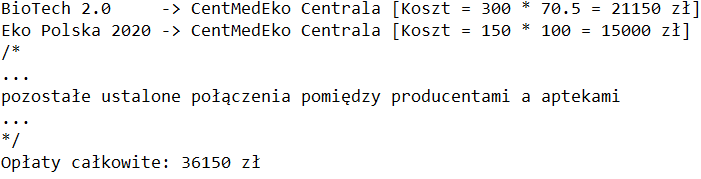
\includegraphics{out.png} 
\end{enumerate}
 
  \item Opis klas
  
  \begin{enumerate}[label=\arabic{enumi}.\arabic*.]
  \item Loader\\
  
 Klasa ta jest częścią pakietu $load$. Nie dziedziczy po żadnej klasie, nie implementuje też żadnych interfejsów. Importuje java.io.FileNotFoundException,  java.io.FileReader oraz java.io.IOException. Zadaniem tej klasy jest zapisanie danych z pliku do utworzonych macierzy.\\
W konstruktorze tej klasy wywołuję metodę tworzące FileReadera i zapisującą informacje z niego pozyskane w postaci macierzy. W klasie znajdują się 2 zmienne będące macierzami.\\
 \textbf{Metoda read}\\
Nagłówek: public void read(string fileName)\\
Zadanie: tworzy obiekt klasy FileReader i przypisuje go do odpowiedniego pliku podanego jako argument tej metody, następnie wywołuje metodę ustawiającą dane w macierzach.\\
Co zwraca: Funkcja typu void, czyli nic nie zwraca.\\
 \textbf{Metoda getConnections}\\
Nagłówek: public int[][] getConnections()\\
Zadanie: getter macierzy z połączeniami\\
Co zwraca: macierz z połączeniami\\
 \textbf{Metoda getDaS}\\
Nagłówek: public int[][] getDaS()\\
Zadanie: getter macierzy popytem i podażą\\
Co zwraca: macierz z popytem i podażą\\
 \item Aprox\\
Klasa jest trzonem pakietu $aprox$.Nie dziedziczy po żadnej klasie, nie implementuje też żadnych interfejsów. Zadaniem tej klasy jest operowanie na utworzonych macierzach w taki sposób, aby korzystając z pomocy trzeciej macierzy zoptymalizować proces zakupu szczepionek i wybrać jak najmniejszą cenę.\\
W konstrukorze tej klasy korzystam z dwóch macierzy przekazywanych jako argumenty wywołania w celu wywołania metody tworzącej trzecią macierz oraz wywołuję metodę aproksymującą.
 \textbf{Metoda remainingDaS}\\
Nagłówek: public int[][] remainingDaS(int[][] connections, int[][] das)\\
Zadanie: stworzenie macierzy z pozostałym zapotrzebowaniem i dostępnymi szczepionkami\\
Co zwraca: macierz z pozostałym zapotrzebowaniem i dostępnymi szczepionkami\\
 \textbf{Metoda vam}\\
Nagłówek: public int[][] vam(int[][] connections, int[][] das)\\
Zadanie: stworzenie macierzy obrazującej ile szczepionek od każdego z dystrybutorów zostało sprzedanych danej aptece. Wykorzystany będzie algorytm VAM.\\
Algorytm: VAM polega na kolejnym znajdowaniu różnicy między dwoma najmniejszymi wartościami w każdej kolumnie i każdym wierszu. Następnie wybierana jest największa liczba spośród tych różnic. Jeżeli liczba ta jest różnicą pochodzącą wartości w jednej kolumnie, to oznacza to, że w tej kolumnie zostanie zawarta pierwsza transakcja. Jeżeli transakcja wyczerpuje podaż lub popyt, to wtedy do dalszych akcji nie jest brany pod uwagę dany producent(dostawca) lub apteka. Akcja ta jest powielana do momentu zospokojenia potrzeb wszystkich aptek(odbiorców).
Co zwraca: macierz obrazującą, który producent sprzedał ile szczepionek danej aptece.\\
\item Main \\
Klasa ta należy do pakietu $aprox$. Nie dziedziczy po żadnej klasie, nie implementuje interfejsów. Jedynym zadaniem tej klasy jest posiadanie metody main, w której tworzone są obiekty pozostałych klas i wywoływane są ich metody.
\item ResultsSaver \\
Klasa ta należy do pakietu $save$. Nie dziedziczy po żadnej klasie, nie implementuje interfejsów. Zadaniem tej klasy jest stworzenie pliku $result.txt$, a następnie zapisanie do niego danych. Importuje java.io.FileWriter oraz java.io.IOException. W konstruktorze tworzę nową instancję obiektu FileWriter z argumentem $result.txt$. 
 \end{enumerate}

\item Testowanie
\begin{enumerate}[label=\arabic{enumi}.\arabic*.]
 \item Użyte narzędzia 
Testy wykonałem używając JUnit 4.
 \item Konwencja testów
Nazwy testów sugerują, co powinno być zwracane w danej metodzie. Przykładem jest shouldRaiseWrongTextFormatError.
\item Warunki brzegowe
Zdecydowanie najwięcej błędów może występować przy wczytywaniu danych z pliku. Tutaj będzie najwięcej testów, jeden test dla każdego typu błędu. Testy będą też dotyczyły samej aproksymacji VAM.
 \end{enumerate}	

 \end{enumerate}

\end{document}